% !TeX root = ../main.tex
\section{V4：证据约束的代码生成与单循环决策}
\label{sec:v4-method}
\subsection{研究问题与总体结构}
V3 的有限任务结果尚未回答一个更开放的问题：当用户需求不能由既有工具中的固定算法直接表达时，系统能否生成新的任务程序，并保持原始科学目标与验证条件？V4 以此为中心，将任务表达从工具参数扩展到现场生成的 Python 和 ORCA 输入。Code as Tools 的基本原则是：任务特定算法由代码表达，通用工具承担校验、执行和产物管理。

V4 采用一个决策主循环。模型根据当前目标、计划和证据提出下一动作；程序检查依赖、资源和执行边界后调用工具；新结果先接受科学检查与目标评价，再反馈至下一轮决策。计算正常结束后仍可能需要精度检查、补充采样或跨结果分析，失败则可能引出输入修复或有原因的停止。该组织不预设优化、频率与单点的固定顺序。

\begin{figure}[H]
\centering
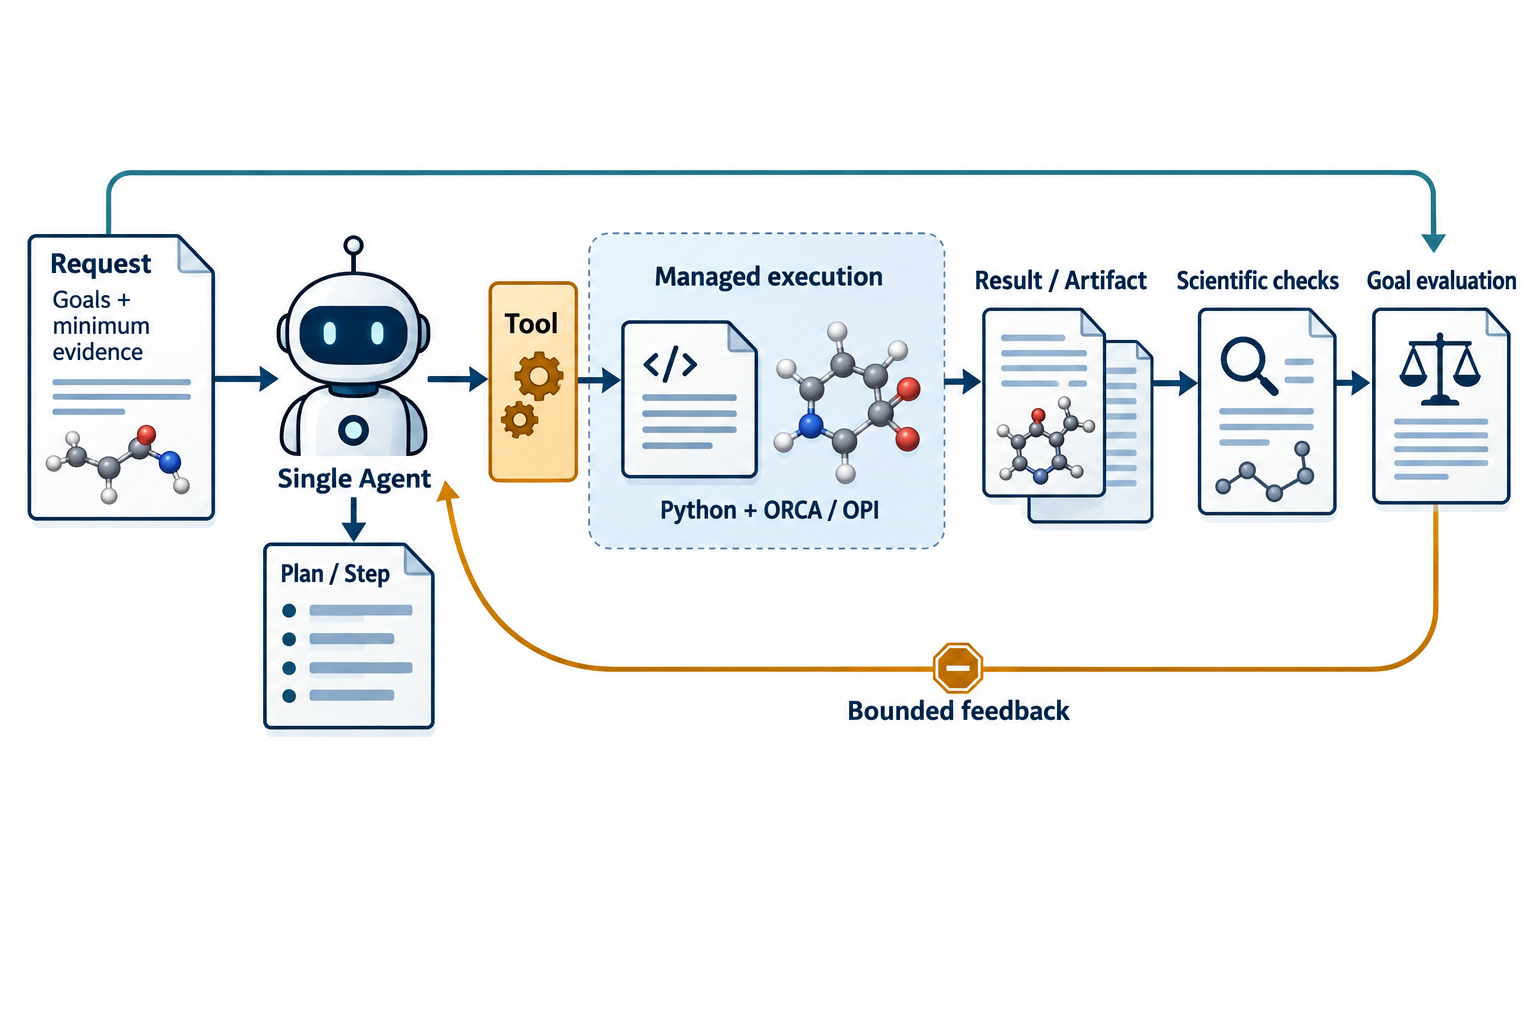
\includegraphics[width=\linewidth,trim=14 205 14 112,clip]{method-overview.png}
\caption{V4 的证据约束闭环。原始目标独立约束结果评价；单一决策者通过工具边界组织计算，依据新证据修订执行路线。该图为方法示意。}
\label{fig:architecture}
\end{figure}

\subsection{领域表示与目标保持}
系统采用 Request、Plan、Step、Tool、Run、Result 和 Artifact 七类长期对象，分别表达科学需求、实现路线、具体步骤、执行接口、运行过程、结果与证据产物。表 \ref{tab:objects} 给出其功能关系。该表示将目标语义、执行状态和科学结果分离，避免由单一“成功”标记覆盖不同层次的事实。

\begin{table}[htbp]
\centering\small
\caption{V4 的核心表示及其方法作用。}
\label{tab:objects}
\begin{tabularx}{\linewidth}{p{1.8cm}YY}
\toprule
对象 & 主要内容 & 方法作用\\
\midrule
Request & 科学对象、物理量、条件、最低证据 & 固定任务所要回答的问题\\
Plan & 步骤依赖、目标到证据的路线 & 允许调整实现策略\\
Step & 工具参数、输入或代码版本 & 明确一次具体操作\\
Tool & 接口约束、执行影响、检查与产物 & 建立可验证的执行边界\\
Run & 配置、尝试、资源与累计用量 & 保持运行连续性与有限成本\\
Result & 执行事实、科学检查、观察与目标评价 & 区分结果层次\\
Artifact & 几何、输入、程序、原始输出与来源 & 支持追溯和复核\\
\bottomrule
\end{tabularx}
\end{table}

目标和最低证据保存在 Request 中，Plan 仅负责实现路线。例如，将“在同一几何上比较气相与水环境能量”修订成两套独立优化，虽然可能产生两个数值，却改变了原问题。不同目标允许具有不同环境或电子态，实际执行条件因而需要按目标匹配，而不能无条件归并为全局设置。

修复同样受到目标保持约束。当某个程序因语法或输入错误而修改时，未改变的目标路线应保持关联；修复不能通过删除目标或降低最低证据要求获得形式上的完成。用户明确条件、默认值、继承条件与自动选择分别记录，以便区分模型决策和外部约束。

\subsection{统一执行入口与任务算法生成}
V4 支持三种输入形式：OPI 构造的输入、原生 ORCA 输入，以及生成 Python 通过薄接口发起的内部计算请求。三者复用相同的 ORCA 执行管理与既有解析、检查链，OPI 接口行为以其版本化文档为依据\cite{opi}。薄接口负责请求计算和返回产物引用，不内置构象搜索、势能扫描等具体解题算法。

因此，开放性主要来自任务程序的组合能力。一个程序可以构建几何集合、选择有限候选、提交内部计算，并在结果产生后执行确定性分析。相同通用工具可被用于不同性质或数据组织方式，减少为每个问题增加专用求解接口的需要。这一机制扩展的是表达能力，其科学有效性仍需按输出检查。

模型负责提出意图、参数、代码和修复建议，程序负责判定是否可执行。生成代码不能自行扩展权限、修改系统实现或宣告科学通过。工具目录、参数定义、执行校验与输出声明保持一致，以减少规划接口与实际行为之间的不一致。

\subsection{开放观察与科学资格}
新任务可能产生尚未纳入标准检查的性质。V4 允许代码从原始输出提取此类数据，并将其记录为带来源、单位和验证说明的观察。这有助于支持开放分析，但观察不会自动成为经过科学检查的正式结果。程序退出码、字段存在或脚本给出的“通过”均不足以替代性质相关验证。

对于标准检查已覆盖的输出，系统沿用统一解析与科学检查；对于未覆盖的输出，则披露其证据状态及结论边界。是否足以满足目标取决于原请求的最低要求，而不是模型对结果的主观评价。该区分尤其适用于激发态、张量性质和由多个计算派生的结论。

原始输入、初始几何和历次尝试保持独立；结果引用通过内容校验绑定相应产物。读取已有证据不隐式触发转换或重算，额外分析和补算作为明确操作进入决策过程。这样既保留失败事实，也使成功结果能够被后续步骤可靠消费。

\subsection{有界反馈、资源与停止机制}
开放代码引入了动态计算数量与程序行为，因此资源与预算需要覆盖整个任务，而不只约束最外层调用。对预算维度 $k$，令上限为 $B_k$、累计用量为 $U_k$、新动作预留为 $r_k$，执行前要求
\begin{equation}
U_k+r_k\leq B_k.
\end{equation}
内部 ORCA 调用、代码重试与模型纠错均计入累计用量；运行恢复不重置消耗。执行状态不明时先核对既有运行事实，避免重复启动。

生成程序及其科学子进程处于受管理的执行范围中，共同受到计算资源、文件访问和通信约束。本文评估所采用的环境计算并发为 1，使用 4 核、进程树内存上限 1024 MiB 和 ORCA MaxCore 192 MiB/进程。MaxCore 是程序内部参数，不能替代总内存限制。既有隔离测试仅支持已评估配置，不能推导任意环境下的安全性。

反馈内容需在有限上下文内同时保留原始目标、当前结果和有效修复信息。V4 采用当前证据摘要与可查询来源相结合的组织方式。预算耗尽、证据不足或不适用均可构成停止理由；停止后已经正常结束的 ORCA 调用保留计算成功标记，其科学解释与工作流交付状态分别记录。
